


\chapter{Was sind Microservices?}\label{sec:microservices}

Prinzipiell ist es schwierig Microservices einheitlich zu definieren. Gründe dafür sind zum einen, dass das Prinzip von Microservice-Architekturen zwar klar ist, es aber dennoch unterschiedliche Ansichten und Verständnisse  diesbezüglich in der Fachliteratur gibt. Zum anderen gibt es keine einheitliche Architektur von Microservices, bzw. das Grundprinzip ist klar, dies wird allerdings unterschiedlich umgesetzt. Genaueres zu der uneinheitlichen Architektur von Microservices wird in \ref{sec:funktionsweise} beschrieben.\newline\newline 

„Eine Microservicearchitektur besteht aus einer Sammlung kleiner, autonomer Dienste. Jeder Dienst ist eigenständig und sollte eine einzige Geschäftsfunktion implementieren.“\cite{microsoft}\newline\newline 

„Die Microservice-Architektur - oder einfach nur Microservices - ist eine eigene Entwicklungsmethode für Softwaresysteme, die sich auf die Entwicklung von Modulen mit nur einer Funktion mit gut definierten Schnittstellen und Operation zu konzentrieren versucht.“\cite{smartbear}\newline\newline 

„A microservice, in my mind, is a small application that can be deployed independently, scaled independently, and tested independently and that has a single responsibility. It is a single responsibility in the original sense that it's got a single reason to change and/or a single reason to be replaced. But the other axis is a single responsibility in the sense that it does only one thing and one thing alone and can be easily understood.“\cite{ieeetalk}\newline\newline 

Man sieht, das es keine standardisierte, formalisierte Definition von Microservices gibt. Dennoch gibt es grundlegende charakteristische Merkmale die diese Architektur beschreiben.\newline
Microservices ist eine Methode zur Entwicklung von Softwareanwendungen als Umgebung von unabhängigen, voneinander einsetzbaren, modularen Diensten. Jeder Service soll so konfiguriert sein, das er als alleiniger Dienst ausgeführt werden kann, Daten unabhängig von anderen Diensten verarbeitet und nur über genau definierte Schnittstellen mit anderen Services kommuniziert.\cite{keyhole}\newline

Genauer gesagt Microservice ist ein Ansatz zur Modularisierung von Software. Das heißt große Software-Systeme sollen in kleine Module unterteilt und entwickelt werden.\newline
Dadurch soll es möglich sein Software einfacher zu erstellen, zu verstehen und weiterzuentwickeln. Des Weiteren sollen Microservices möglichst klein, unabhängig und lose gekoppelt sein. Ein Dienst wird von einem kleinen Entwicklerteam geschrieben und verwaltet. Microservices werden unabhängig von einander bereitgestellt, getestet und deployt.\newpage 

Das Konzept des Microservice verfolgt den gleichen Ansatz wie die Unix-Philosophie\cite{unixphilosophie}\newline
\begin{description}
 \item - Ein Programm soll genau eine Aufgabe erledigen. Diese soll aber richtig erledigt werden.
 \item - Programme sollen zusammen arbeiten können.
 \item - Es sollen universelle Schnittstellen genutzt werden.
\end{description}


\chapter{Wie funktionieren Microservices?}\label{sec:funktionsweise}

Wie schon im vorherigen Abschnitt erwähnt sind Microservices modular aufgebaut und sollen nur über geeignete Schnittstellen miteinander/mit dem Programm kommunizieren. Daher wird jeder Microservice auf einem eigenen Server betrieben, wobei die Services voneinander nichts wissen sollen. Die Funktionsweise bzw. der genaue Ablauf eines Microservices wird in \ref{sec:funktion} beschrieben.\newline\newline

\begin{figure}[bth]
    \centering
    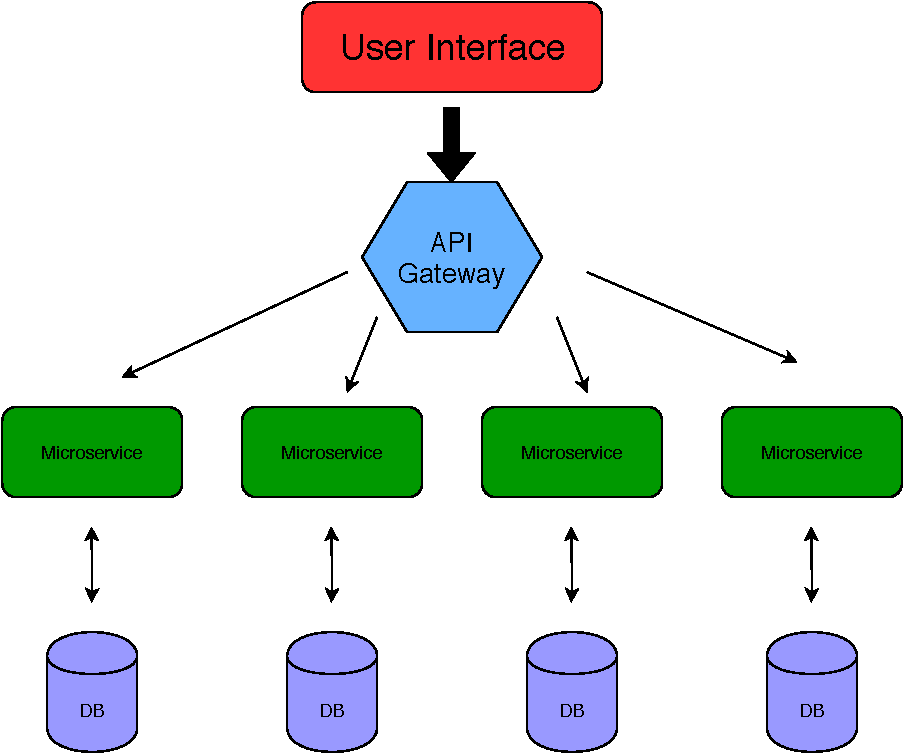
\includegraphics[width=0.8\textwidth]{Chapters/Bilder/Microservices.pdf}
    \caption{Microservice}
   \label{fig:microservice}
  \end{figure}
  
\newpage

\ref{fig:microservice} zeigt einen grundlegenden Aufbau eines Microservices. Wie im vorherigen Abschnitt erwähnt ist es schwierig eine einheitliche Architektur für Microservices zu definieren. Dies wird im folgenden Abschnitt beschrieben.
Wie man dennoch zu einer guten Architektur kommt, die auf die Organisation und oder das Programm passt und welche Herausforderungen dabei beachtet und bewältigt werden müssen wird in \ref{ch:Herausforderungen} beschrieben.\newline\newline

Vom Grundgedanken her besitzt jeder Microservice sein eigenes User Interface, durch welches der Nutzer mit der Software kommunizieren soll. Da Microservices allerdings modular aufgebaut sind und im besten Fall unabhängig von einander sind müssen die einzelnen User Interfaces der Microservices noch einmal in einer großen Master IU zusammen gefasst werden. Diese Master UI dient dazu, die einzelnen User Interfaces der Microservices zu bündeln und dem Nutzer so eine UI zur Verfügung zu stellen, sodass es den anschien hat das es eine einzige UI ist. Dieser Architektur-Ansatz wird allerdings eher selten in der Praxis genutzt, da es ohne ausreichender Kommunikation unter den Teams bzw. ohne eines grundlegenden Designs der Oberfläche zu Inkonsistenz und unterschiedlich aussehenden Bausteinen der UI kommen kann.
Daher wird bei der Erstellung von Microservices eher auf den Aufbau wie in \ref{fig:microservice} zurückgegriffen, d.h es gibt ein gemeinsames User Interface das von einem Team erstellt und verwaltet wird. Dadurch entsteht zwar im Umkehrschluss eine erhöhte Kommunikation der einzelnen Microservice Teams und des UI Teams, wenn neue Features implementiert werden müssen. Allerdings ist auf der anderen Seite eine einheitliche und runde Oberfläche gewährleistet. Dies ist gerade für den Endnutzer von Vorteil, da er dadurch ein angenehmeres Gefühl bei der Arbeit mit der Software hat.\newline\newline

Wie am Anfang des Abschnitts beschrieben liegt jeder Microservice auf einem eigenen Server und kann nur über eine Schnittstelle nach außen kommunizieren. An dieser Stelle kommt das API-Gateway ins Spiel.
Das API-Gateway dient als Einstiegspunk für die Clients. Das bedeutet anstatt den Service direkt aufzurufen, rufen die Clients das API-Gateway auf. Dieses leitet anschließend den Aufruf an den geeigneten Service im Back-End weiter.  Dies hat unter anderem die Vorteile, dass\cite{microsoft}:
\begin{description}
	\item - Es entkoppelt die Clients von den Diensten. Für Dienste kann eine Versionierung oder Umgestaltung durchgeführt werden, ohne dass sämtliche Clients aktualisiert werden müssen. 
	\item - Dienste können nicht web fähige Messagingprotokolle verwenden, z.B. AMQP. (Was ist das)
	\item - Das API-Gateway kann weitere übergreifende Funktionen ausführen, beispielsweise Authentifizierung, Protokollierung, SSL-Terminierung und Lastenausgleich.
\end{description}

Allerdings ist das API-Gateway kein Muss bei der Implementierung einer Microserice-Architektur sondern eine Möglichkeit seine Architektur übersichtlicher zu gestalten. Gerade bei kleineren Software-Systemen kann man auf ein API-Gateway verzichten und die Kommunikation zwischen UI und Microservice über Frameworks wie zum Beispiel REST gestalten. Diese Art der Kommunikation wird auch im Kapitel \ref{ch:Fallstudie} genutzt, um zu zeigen wie solch eine Architektur in einem System funktionieren kann.\newpage


Jeder Microservice hat seine eigenes Back-End in dem die Bussines-Logic enthalten ist. Dort wird genau eine Funktionalität implementiert und es soll möglichst darauf geachtet werden das kein Service von anderen Services abhängig ist geschweige denn Funktionalitäten von anderen Services enthält. Auf dieses Problem wird noch einmal genauer in Kapitel \ref{ch:Herausforderungen} eingegangen, wie damit umzugehen ist.\newline\newline

Prinzipiell hat jeder Microservices seine eigene Datenhaltungsschicht auf die nur er zugreifen kann/soll. Allerdings gibt es auch Ansätze bei denen sich mehrere Microservices eine gemeinsame Datenhaltung teilen bzw. auf mehrere Datenhaltungen zugreifen. Dieser Ansatz wird auch in \ref{ch:Fallstudie} genutzt. 
Welche Art der Datenhaltung genutzt wird, sollte Projekt und Architekt abhängig betrachtet werden, da es bei Zugriffen von mehreren Services auf dieselbe Datenhaltung schnell zu Problemen kommen kann. Welche Probleme an dieser Stelle genau auftreten können und wie diese zu lösen sind wird genauer in \ref{ch:Daten} beschrieben.

\section{Funktionsweise}\label{sec:funktion}

Ein Client nutzt die Software welche aus einer Microservice-Architektur besteht. Über das User-Interface kann er mit dem System kommunizieren. Möchte er nun eine Funktionalität der Software nutzen, wird zuerst die Anfrage an das API-Gateway geleitet. Dieses schaut welche Microservices für diese Anfrage zuständig sind und leitet anschließend die Anfrage an den/die entsprechenden Services weiter. Diese bearbeiten die Anfrage und geben das Ergebnis zurück an das API-Gateway sodass das Ergebnis nun auf der UI dargestellt werden kann. Die genaue Kommunikation kann zum Beispiel über eine REST-Schnittstelle laufen welche JSON-Objekte empfängt und versendet.

\chapter{Vergleich mit anderen Architektur-Stilen}

In diesem Abschnitt beschäftigen wir uns mit dem Vergleich der Microservice-Architektur gegenüber dem herkömmlichen Architektur-Stil des Monolithen, sowie der ähnlich aufgebauten Architektur der Service Oriented Architecture. Kurz SOA.
Dabei wird zuerst darauf geschaut was sich hinter diesen beiden Architektur-Stilen verbirgt und wie diese funktionieren. Anschließend wird ein Vergleich zwischen dem Microservices und der jeweiligen Architektur gezogen.

\section{Vergleich Monolith}

Um zu schauen in wie fern sich die Architektur eines Microservice mit der Architektur eines Monolithen unterscheidet, muss zuerst geklärt werden was unter einem Monolithen verstanden wird.\newline\newline

Ein Monolith ist ein Software-System welches als eine große untrennbare Einheit gestaltet wird. Die monolithische Architektur folgt keiner expliziten Gliederung in Teilsysteme sondern wird als ein ganzes Software-System betrachtet.\cite{monolith}
Dieses Software-System, häufig auch als Legacy-System bezeichnet, besteht im Endeffekt aus einer  einzelnen logisch ausführbaren Datei. Diese beinhaltet die gesamte Logik der Software und wird serverseitig verwaltet. Die Software läuft meist in einem einzigen Prozess auf einem Server, auf den von außerhalb zugegriffen werden kann. 
Da es sich bei dem Monolithen um eine ausführbare Datei handelt, muss bei jeder Änderung an dem System der Aufbau und die Bereitstellung einer neuen Version, für die serverseitige Anwendung gewährleistet sein.\cite{fowlerlewis}

\begin{figure}[bth]
    \centering
    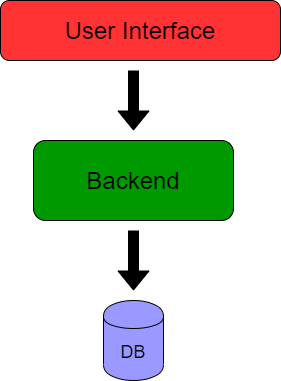
\includegraphics[width=0.4\textwidth]{Chapters/Bilder/Monolith.png}
    \caption{Monolith}
   \label{fig:monolith}
  \end{figure}
  
\ref{fig:monolith} zeigt den prinzipiellen Aufbau und die Funktionsweise eines Monolithen.
Dieser ist in drei Schichten aufgeteilt: dem User Interface, der Backend und der Datenhaltungsschicht.
Das User Interface bietet die Möglichkeit der Kommunikation mit dem System. Es empfängt Ereignisse und leitet diese an das Backend weiter.
Im Backend befindet sich die gesamte Business-Logik des Software-Systems. Es verarbeitet die empfangenen Nachrichten und greift auf die entsprechend benötigten Daten in der Datenhalten zu.
Die Datenhaltungsschicht beinhaltet alle benötigten Daten die das Software-System verarbeitet.\newline\newline

Vergleicht man nun die Architektur des Microservices mit der Architektur des Monolithen gibt es auf der einen Seite Ähnlichkeiten in Bezug auf die einzelnen Komponenten.\newline
Man könnte sagen das jeder Microservice ein sehr kleiner Monolith sei, da jeder Microservice je nach Architektur sein eigenes User Interface besitzt. Ein eigenes Backend sowie eine eigene Datenhaltung hat. Dies steht aber im Widerspruch mit der Bedeutung eines Monolithen, bei dem es sich um eine große Einheit handelt und ein Microservice meist nur aus wenigen Funktionalitäten. Dennoch ist der Vergleich naheliegend.\newline
Im Vergleich zu dem Monolithen liegen die einzelnen Microservices auf unterschiedlichen Servern, wodurch die Kommunikation über spezielle Schnittstellen umgesetzt wird, welche über das Internet miteinander kommunizieren. Bei einem Monolithen ist dies nicht der Fall, da die gesamten Funktionalitäten auf einem Server liegen und dadurch direkt aufgerufen werden können. Auch die Datenhaltung unterscheidet sich bei einem Microservice und dem Monolithen, da jeder Microservice meist seine eigene Datenhaltung besitzt und ein Monolith meist nur auf eine oder wenige Datenhaltungen zugreift.\newline
Ein wesentlicher Unterschied zwischen den beiden Architektur-Stilen ist der Umgang mit Abhängigkeiten. Da jeder Microservice auf einem eigenen Server läuft und nur für einen einzige Funktionalität zuständig ist, ist es wichtig das wenige, im Idealfall, keine Abhängigkeiten zwischen Microservices entstehen, da dies zu erheblichen Problemen führen kann. Genaueres zu dieser Problematik in Kapitel \ref{ch:Herausforderungen}.\newline
Bei einem Monolithen sollte zwar auch Wert auf eine saubere Architektur gelegt werden und dadurch sehr genau auf Abhängigkeiten geachtet werden. Dennoch ist es an dieser Stelle nicht so gravierend bzw. Abhängigkeiten werden sogar benötigt. 
Ein weiterer Unterschied ist die Aufteilung der Entwicklerteams. Bei einem Monolithen werden die Teams auf der technischen Ebene aufgeteilt. Das heißt, ein Team ist für die Datenhaltung zuständig, ein anderes Team kümmert sich um die Business-Logik und ein weiteres Team ist für die graphische Oberfläche verantwortlich.\newline
Bei einem Microservices werden die Teams nach Fachlichkeit des Geschäftsprozesses aufgeteilt. \newline
Hier ist ein Team zum Beispiel für die Artikelsuche eines Online-Shops zuständig. Ein weiteres für den Warenkorb und ein drittes Team für den Kaufabschluss. Dadurch ist jedes Team für einen Geschäftsprozess alleine verantwortlich und muss sich sowohl um die Nutzeroberfläche als auch um die Business-Logik und die Datenhaltung kümmern.\newpage


\section{Vergleich SOA}

Schaut man sich die beiden Architektur-Stile Microservice und SOA an, scheinen sie auf dem ersten Blick recht identisch zu sein. Bei beiden Ansätzen steht die Aufteilung großer Systeme in kleinere Services im Vordergrund. Daher werden in der Literatur Microservices und SOA häufig als dasselbe bezeichnet, da sich beide Ansätze mit der Aufteilung von Anwendungen in Services beschäftigen. Schaut man sich die beiden Ansätze nun aber genauer an stellt man fest, das sie sich in bestimmten Punkten weit aus mehr unterscheiden als zuvor angenommen.\cite{microservices}

Für Service Oriented Architecture oder kurz SOA  gibt es, wie für Microservices, keine einheitliche Definition. Dennoch gibt es zentrale Bestandteile dieser Architektur, welche große Ähnlichkeiten mit Microservices aufweisen. 
Unter anderem besteht SOA wie Microservices aus Services welche eine Funktionalität umfassen sollen, sowie das der Service eigenständig genutzt werden kann. Des weiteren sollen die Services über das Internet und über eine geeignete Schnittstelle miteinander kommunizieren. Auch ist die Nutzung von verschiedenen Programmiersprachen sowie Frameworks bei der Entwicklung von SOA möglich.\cite{microservices}\cite{soa}

\begin{figure}[bth]
    \centering
    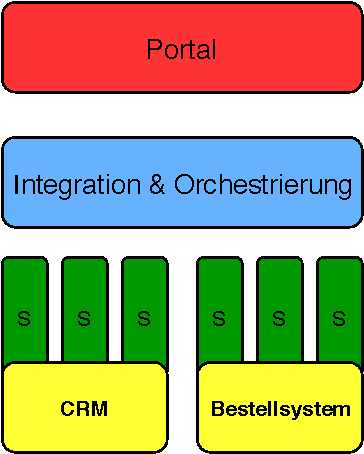
\includegraphics[width=0.4\textwidth]{Chapters/Bilder/SOA.pdf}
    \caption{SOA}
   \label{fig:soa}
  \end{figure}
  
\ref{fig:soa} zeigt einen möglichen Architekturansatz und die Funktionsweise eines SOA-Systems. SOA besteht aus einem Portal, einer Integrations- und Orchestrierungsschicht sowie aus mehreren größeren Services welche zu einer bestimmten Fachlichkeit des Geschäftsprozesses gehören. Jeder Service besteht noch einmal aus mehreren kleineren Services.\newline
Das Portal ist vergleichbar bzw. das gleiche wie ein User Interface welches bei den beiden anderen Ansätzen zum Einsatz kommt. Es ist dafür zuständig, Nutzern eine Oberfläche zu bieten, mit der die Services verwendet werden können. Es können auch mehrere Portale koexistieren, jeweils für unterschiedliche Nutzer des Systems. Zum Beispiel für Kunden, den eigenen Support oder auch interne Mitarbeiter wie Verwaltung oder Management. Aber auch für unterschiedliche Plattformen wie Desktop oder mobile Apps. Egal welche Art von Portal, für die Architektur macht dies keinen Unterschied.\newline
In der Integrations- \& Orchestrierungsschicht sind die einzelnen Services in einem Verzeichnis registriert. Sie übernehmen die Anfragen der Clients, suchen nach den entsprechenden Services die für dies Anfrage benötigt werden und rufen diese mit den entsprechenden Daten auf.\newline
Die größeren Services sind wie schon erwähnt in Fachlichkeiten des Geschäftsprozesses unterteilt und beinhalten wiederum mehrere kleinere Services, vergleichbar mit Microservices, welche zu Umsetzung einzelner kleinere Geschäftsprozesse dienen. Als Beispiel beinhaltet ein Service das Customer Relationship Management (CRM), welches sich um die Kundenverwaltung kümmert. Die einzelnen Services sind dann für die einzelnen Prozesse des CRM zuständig wie zum Beispiel, Kunde registrieren, Kunde löschen oder Kunde ändern. Jeder größere Service beinhaltet eine eigene Datenhaltung, auf die, die einzelnen Services zugreifen können.\newline\newline

Vergleicht man nun beide Ansätze stellt man fest, das es wie schon erwähnt viele Gemeinsamkeiten gibt, aber auch große Unterscheide, wodurch es schwierig wird Microservices und SOA als das gleiche zu betrachten.\newline
Beide Ansätze streben die Aufteilung von Anwendungen in Services an, sowie die Kommunikation der einzelnen Services über das Netzwerk.\newline
Aber schon bei der Kommunikation bzw. der Integration fangen die Unterschiede an. Bei SOA funktioniert die Integration auch für Orchestrierung. An dieser Stelle wird ein Geschäftsprozess aus den einzelnen Services zusammengesetzt. Die Orchestrierung soll so eine gewisse Flexibilität in das Programm bringen. Bei Microservices hat die Integrationslösung keine eigene Intelligenz. Die einzelnen Services kommunizieren untereinander und müssen sich kennen. Microservices versuchen hingegen die Flexibilität durch einfache und schnelle Änderung sowie Ersetzung von Services zu gewährleisten.\newline
Ein weiterer Unterschied ist die Aufteilung der Teams in Fachlichkeit und Technik.
Bei SOA gibt es ein Team welches für die Oberfläche bzw. das Portal zuständig ist. Ein Team welches sich um die Integration \& Orchestrierung kümmert. Diese beiden Teams sind auf technische Weise aufgeteilt. Andere Teams kümmern sich um die einzelnen fachlichen Aspekte des Systems, wobei diese für eine Sammlung von Services des jeweiligen Geschäftsprozesses zuständig sind. Durch die Integration und Orchestrierung muss eine unternehmensweite Integrationslösung eingeführt werden, da es gerade bei dem Zugriff auf Daten zu Problemen führen kann. Bei Microservices ist dies leichter zu handhaben, da es keine einheitliche Integrationstechnologie gibt. Die Technologie der Integration und Kommunikation ist auf den Service begrenzt. Gerade bei Datenreplikationen ist dies von Vorteil. Genaueres hierzu in \ref{ch:Daten}.\newline
Auch die Kommunikation zwischen mehreren Teams ist bei SAO schwieriger als bei Microservices. Durch die Aufteilung auf technischer Ebene kann es bei Änderungen eines Service dazuführen, das Anpassungen an anderer Stelle, für die ein anderes Team verantwortlich ist, getätigt werden müssen. So muss zum Beispiel bei der Änderung eines Services auch die Oberfläche entsprechend geändert werden, wodurch das Team Service mit dem Team Portal kommunizieren muss.\cite{microservices}

\chapter{Warum nutzt man Microservices?}

In diesem Abschnitt wird darüber gesprochen, wieso es sinnvoll ist eine Microservice-Architektur zu verwenden und welche spezifischen Vorteile solch ein Architektur Ansatz mit sich bringt.
In den vorherigen Abschnitten wurde bereits ein Teil der Vorteile leicht angeschnitten. Nun werden diese detaillierter dargestellt.
Da es sich bei den Vorteilen nicht nur um technische Aspekte handelt, werden diese in drei Kategorien unterteilt:
\begin{description}
	\item - Technische Vorteile
	\item - Organisatorische Vorteile
	\item - Geschäftliche Vorteile
\end{description}

\section{Technische Vorteile}

Wie schon in den vorherigen Abschnitten erwähnt sind Microservices modular aufgebaut und jeder Service liegt auf einem eigenen Server. Dadurch entsteht eine verteilte Kommunikationsstruktur. Diese ermöglicht es einem Service, mit anderen Services zu kommunizieren bzw. diese aufzurufen. Diese Kommunikationsinfrastruktur muss dementsprechende Möglichkeiten enthalten um die Kommunikation zwischen den Services zu ermöglichen. Ein Entwickler muss diese Infrastruktur genau beschreiben. Dadurch ist es schwieriger das Abhängigkeiten zwischen zwei oder mehreren Services entstehen, da der Entwickler diese explizit einbauen muss, um die Kommunikation zu gewährleisten. Falls sich doch einmal solch eine Abhängigkeit ungewollt einschleichen sollte, gibt es  spezielle Architekturmanagement-Werkzeuge um diese zu finden. Gerade bei Microservices ist dies leicht zu korrigieren, wenn man die Abhängigkeit frühzeitig entdeckt, da der Service schnell abgeändert werden kann oder komplett neu geschrieben werden kann. Genaueres zu dem Umgang mit Abhängigkeiten wird im Kapitel \ref{ch:Herausforderugen} beschrieben.\cite{microservices}\newline\newline

Ein weiterer Vorteil ist wie gerade beschrieben, die mögliche Ersetzung eines Microservices.
Gerade der Umgang mit alten Software-Systemen ist eine große Herausforderung. Oftmals ist die Codequalität recht schlecht, da die Software über Jahre hinweg von unterschiedlichen Entwicklern weiter entwickelt wurde und an vielen Stellen Hilfen eingebaut wurden, um temporäre Probleme zu lösen, die der Entwickler später wieder beheben wollte, dies aber nie tat. Diese Software weiter zu entwickeln oder gar neu zu schreiben ist ein fast unmögliches Unterfangen, da an vielen Stellen gar nicht mehr bekannt ist was einzelne Funktionen oder Codeabschnitte genau machen und der Entwickler der sie geschrieben hat, nicht mehr in dem Unternehmen tätig ist. Je größer die Software ist, desto größer ist der Aufwand. Beinhaltet die Software zusätzlich noch wichtige Geschäftsprozesse ist es praktisch unmöglich die Software noch zu ändern, da ein Ausfall der Software einen erheblichen finanziellen Schaden bedeuten kann.\newline
Microservices bieten an dieser Stelle den Vorteil das die Entwickler zum einen nicht an bestimmte Technologien gebunden sind, sondern können beliebige andere Technologien nutzen um das Problem zu lösen. Dadurch das ein Microservice im Idealfall auf der fachlichen Ebene eigenständig agiert, muss nicht genau bekannt sein wie die einzelnen Funktionen genau funktionieren. Dem Entwickler muss nur bekannt sein welche fachlichen Funktionalitäten der Microservices haben soll und welche Geschäftsprozesse er beinhaltet. Danach kann er diesen einfach durch einen neuen Microservice ersetzten.\cite{microservices}\newline\newline

Im Umgang mit Legacy-Systemen bilden Microservices einen weiteren Vorteil. Wie bei dem Vorteil der Ersetzung eines Microservices beschrieben, sind Legacy-Systeme oft recht unübersichtlich je größer sie werden. Mit Hilfe von Microservices können einzelne Codeabschnitte oder Funktionalitäten der Software einfach an einen Microservice ausgelagert werden. Hierzu muss einfach eine Schnittstelle an die Stelle der Funktionalität gebaut werden, welche ersetzt werden soll. Diese leitet die Anfrage anschließend an den Microservice weiter der diese dann verarbeitet. Anschließend kann er das Ergebnis wieder an das Legacy-System zurück senden, welches wiederum mit dem Ergebnis weiter arbeiten kann. Dadurch können kritische, schwer zu ändernde Codeabschnitte gezielt umgangen und ausgelagert werden, ohne das es zu Problemen mit dem System kommt.\cite{microservices}\newline\newline

Continous Delivery brint Software durch einen einfachen reproduzierbaren Prozess regelmäßig in Produktion. Dazu dient eine Continuous-Delivery-Pipeline.

\begin{figure}[bth]
    \centering
    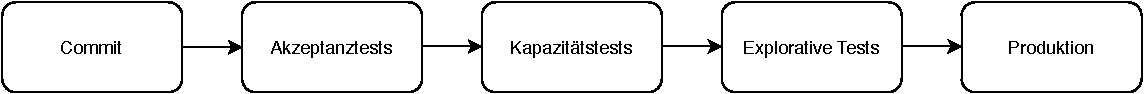
\includegraphics[width=1.0\textwidth]{Chapters/Bilder/CDP.pdf}
    \caption{Continuous-Delivery-Pipeline}
   \label{fig:cdp}
  \end{figure}

\begin{description}
	\item - In der Commit-Phase wird die Software kompiliert, die Unit-Tests werden durchgeführt und es wird gegebenenfalls eine statische Code-Analyse durchgeführt.
	\item - Die automatisierten Akzeptanztests in der nächsten Phase stellen sicher, dass die Software fachlich korrekt ist, sodass sie vom Kunden akzeptiert wird.
	\item - Kapazitätstests überprüfen, ob die Software performant genug ist, um die erwartete Anzahl Nutzer zu unterstützen. Auch diese Tests sind automatisiert.
	\item - Die explorativen Tests hingegen sind manuell und dienen dazu, bestimmte Bereiche des Systems zu testen. Dazu können neue Features zählen oder bestimmte Aspekte wie die Sicherheit des Systems.
	\item - Zum Schluss wird die Software in Produktion gebracht. Auch dieser Prozess ist idealerweise automatisiert.
\end{description}
\newpage
Die Software durchläuft jede einzelne Phase der CDP. Nach jeder erfolgreich abgeschlossenen Phase wird sie in der nächsten Phase weiter getestet. An dieser Stelle kann es passieren, dass die Software eine Phase erfolgreich abschließt, dann aber in der nächsten Phase nicht akzeptiert wird, weil zum Beispiel die Laufzeit zu lange dauert.\newline
Gerade hier liegt der Vorteil bei einer Microservice-Architektur. Microservices sind eigenständige Deployment-Einheiten. Daher können sie unabhängig von anderen Services getestet und in Produktion gebracht werden. Dies hat erhebliche Auswirkungen auf die CDP im Vergleich zum Testen von monolithischen Strukturen.
Der Durchlauf durch die einzelnen Tests ist wesentlich schneller, da nur ein kleiner Microservices in Produktion gebracht wird. Dadurch erhält man schnell Feedback, wodurch der Fehler bzw. das Problem behoben werden kann und sofort wieder getestet wird. Dadurch wird eine Menge zeit gespart. Denn wenn der Entwickler erst nach mehreren Tagen oder Wochen erfährt das sein Code fehlerhaft ist, ist es schwieriger sich wieder in den Code einzuarbeiten und den Fehler zu beheben.\newline
Auch ist der zu testende Aufwand wesentlich bei einem Microservice geringer als bei einem Monolithen. Bei einem Monolithen muss der gesamte Code bei einer Änderung wieder deployed und anschließen ausgeliefert werden. Bei einem Microservice ist es nur der Microservice selbst, ohne das andere Teiler der Software getestet und ausgeliefert werden müssen.\cite{microservices}\newline\newline

Auch in Bezug auf Skalierbarkeit haben Microservices Vorteile. Dadurch das jeder Service auf einem eigenen Server betrieben wird, können mehrere Instanzen des selben Microservice betrieben werden. Das heißt es gibt mehrere Services eines Microservices auf verschieden Servern. Dadurch ist eine gute Skalierbarkeit gewährleistet, da die Last auf mehrere Server verteilt werden kann. Auch ist es dadurch möglich Microservices auf unterschiedlich schnellen Servern laufen zu lassen. So kann jeder Microservice seine eigene Skalierung beinhalten. Des weiteren können so Microservices an verschiedenen Stellen im Netzwerk betrieben werden, um so einen geographische Skalierung zu erzeugen.\newline 
An dieser Stelle kommt auch die Robustheit eines Microservices in Spiel. Prinzipiell sollten Microservices anfälliger für Ausfälle sein, da ein Ausfall nicht nur auf der Hardware-Ebene passieren kann, sondern auch ein Ausfall auf der Netzwerk-Ebene. Um trotzdem eine hohe Verfügbarkeit zu gewährleisten muss eine Art Firewall zwischen den Microservices gebildet werden. Ein Ausfall eines Services darf sich nicht auf andere Services ausbreiten und diese ebenfalls zu einem Ausfall bringen. Hierzu kann zum einen bei einem Ausfall ein Microservice mit einem Default-Wert weiter arbeiten oder an einen anderweitig reduzierten Services weiter geleitet werden. Zum anderen kann wie bei Skalierbarkeit beschrieben, bei einem Ausfall eines Microservices einfach ein anderer Service eingesetzt werden, der die gleicher Funktionalität besitzt. Dies wird solange betrieben bis der ursprüngliche Services wieder verfügbar ist.\cite{microservices}\newline\newline

Wie schon in vorherigen Abschnitten beschrieben herrscht bei Microservices eine Technologiefreiheit. Jeder Services kann in einer anderen Programmiersprache geschrieben sein, mit unterschiedlichen Frameworks zusammen arbeiten oder aber auch an bestehende Sprachen angepasst werden. Dies bietet zum einen den Vorteil, das Funktionalitäten mit bestimmten Anforderungen in dafür geeigneten Sprachen geschrieben werden können. Nehmen wir an es wird viel Wert auf die Laufzeit gelegt, so kann der Service in C oder C++ geschrieben werden. Des weiteren ist es so möglich, leichter Microservices zu ersetzen, da man den Service nicht in der ursprünglichen Sprache ersetzten muss, sondern eine beliebige wählen kann. Falls zum Beispiel ein Service in Python geschrieben wurde und der Entwickler die Firma verlassen hat, kann der Service in einer anderen Sprache neu geschrieben werden, falls sich niemand mit Python auskennen sollte. So kann einiges an Einarbeitungszeit gespart werden. Auch die Arbeitsmoral und Motivation kann dadurch gesteigert werden. Durch die technologische Wahlfreiheit können neue Frameworks oder Sprachen getestet werden, ob diese für das Unternehmen lukrativ sind bzw. ob man diese auch in Zukunft für andere Projekte nutzen kann.\newline Normalerweise würde in einem Unternehmen die Zeit fehlen, das sich Entwickler in neue Technologien einarbeiten können, um zuschauen welchen Mehrwert diese für die Firma haben. Des weiteren sorgt die Möglichkeit der Wahlfreiheit für eine gewisse Abwechslung für die Entwickler. Diese müssen nicht Tag für Tag mit der selben Sprachen etc. arbeiten, sondern können sich auch mit neuen Technologien beschäftigen. Dadurch kann zumindest teilweise ein gewisser Trott vermieden werden und die Mitarbeiter neue Impulse setzten.\cite{microsoft}


\section{Organisatorische Vorteile}

Durch die technische Unabhängigkeit kann ein Team, welches für einen Microservice voll zuständig ist, die Unabhängigkeit komplett ausnutzen. Dadurch wird vor allem die Selbstständigkeit des Teams gestärkt. Des weiteren müssen die einzelnen Teams weniger koordiniert werden, da es zum Beispiel nicht wichtig ist das unterschiedliche Bibliotheken oder unterschiedliche Versionen von Bibliotheken genutzt werden.
Die einzelnen Teams sind dafür verantwortlich welche Architektur welche Sprache und weiches Framework genutzt wird. Daraus folgt aber auch, dass das Team die vollen Konsequenzen tragen muss, falls etwas schief läuft. Dies steigert zum einen die Selbstorganisation und zum anderen werden die Teammitglieder zusätzlich motiviert fokussiert zu arbeiten und ihre Entscheidungen zu reflektieren.\cite{microservices}

\section{Geschäftliche Vorteile}

Die bereits erwähnten Vorteile aus der organisatorischen Sicht führen zu geschäftlichen Vorteilen. Das Risiko der Projekte sinkt, da jedes Team eine hohe Eigenverantwortlichkeit trägt und die Koordinierung zwischen den Teams wird weniger, sodass die Teams effizienter arbeiten können.
Durch die Aufteilung in Mikroservices können die Teams unabhängig von einander an den Services Arbeiten, was eine parallele Arbeit ermöglicht. Teams müssen nicht auf Ergebnisse anderer Teams warten , um selbst an ihren Services weiter arbeiten zu können. Dadurch kann auch eine Skalierung auf der Ebene der Entwicklung erzeugt werden. Auch müssen die einzelnen Teams viel weniger untereinander Kommunizieren, was dazu führt das sie schneller Ergebnisse erzielen und ihr Projekt abschließen.
Folgen für das Unternehmen aus geschäftlicher Sicht, sind zum einen schnellere Ergebnisse was wiederum zu einer Gewinnmaximierung führt. Zum anderen weniger Verwaltungsaufwand was auch wieder zu einer Gewinnmaximierung führt.\cite{microservices}
